\section{Chart::Pareto}
\herv{Name:} Chart::Pareto\\ \\
\herv{File:} Pareto.pm\\ \\
\herv{Requires:}Chart::Base, GD, Carp, FileHandle\\ \\
\herv{Description:} \fett{Pareto} is a \fett{subclass} of Chart::Base.\\
The class Pareto creates a pare-to chart. Pareto plots only one dataset and its labels.\\
\\
\herv{Example:}
\begin{figure}[h]
	\begin{center}
		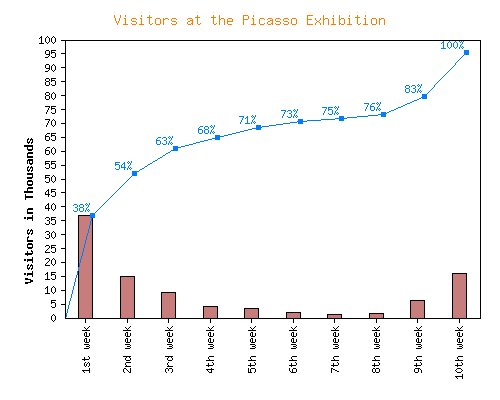
\includegraphics[scale=0.7]{d_pareto2.png}
	\end{center}
	\caption{Pare-to chart}
	\label{fig:pareto}
\end{figure}
\begin{verbatim}
use Chart::Pareto;

$g = Chart::Pareto->new(500,400);
$g->add_dataset ('1st week', '2nd week', '3rd week', '4th week', '5th week',
                 '6th week', '7th week', '8th week', '9th week', '10th week');
$g->add_dataset (37, 15, 9 , 4, 3.5,
                  2.1, 1.2, 1.5, 6.2, 16);

%hash =( 'colors' => { 'dataset0' => 'mauve',
                       'dataset1' => 'light_blue',
                       'title' => 'orange'},
         'title' => 'Visitors at the Picasso Exhibition',
         'integer_ticks_only' => 'true',
         'skip_int_ticks' => 5,
         'grey_background' => 'false',
         'max_val' => 100,
         'y_label' => 'Visitors in Thousands',
         'x_ticks' => 'vertical',
 	       'spaced_bars' => 'true',
         'legend' => 'none'
        );
	
$g->set (%hash); 
$g->png ("pareto.png");
\end{verbatim}
\herv{Constructor:} An instance of a pare-to chart object can be created with the constructor new():\\
\fett{\$obj = Chart::Pareto->new();}\\
\fett{\$obj = Chart::Pareto->new(\kursiv{width}, \kursiv{height});}\\
\\
If \fett{new} has no arguments, the constructor returns an image with the size 300x400 pixels. If new has two arguments \kursiv{width} and \kursiv{height}, it returns an image with the desired size. \\ 
\\ 
\herv{Methods:}All universally valid methods, see page \pageref{methods}: Chart::Base. \\
\\
\herv{Attributes/Options:} All universally valid options, see page \pageref{options}. Also available, these special options:
\begin{description}
\item['y\_axes'] Tells chart where to place the y-axis. Valid values are 'left', 'right' and 'both'. Defaults to 'left'.
\item['spaced\_bars']Leaves space between bars at each data point when set to 'true'.  This just makes it easier to read a bar chart.  Default is 'true'.
\item['sort']Sorts the data descending if set to 'true'. Defaults to 'false'.  
\end{description}